%!TEX root=../GaugeCNNTheory.tex


\subsection{Icosahedral approximations of spherical CNNs}
\label{sec:spherical_CNNs_icosahedral}

The sphere $S^2$ is in computational sciences commonly approximated by Platonic solids, i.e. regular convex polyhedra.
In the context of deep learning, interest has mostly been focused on the icosahedron, Fig.~\ref{fig:ico_neighborhoods}, which approximates the sphere most closely among the platonic solids~\cite{schroder1995spherical}.
While the Riemannian geometry of the sphere is only approximated, Platonic solids have the advantage to be piecewise flat and admit regular meshes.
These properties allow for the use of planar convolution routines, which are computationally better optimized than the methods from the previous two sections.
This section discusses the icosahedral CNNs from~\cite{liu2018icoAltAz}, \cite{zhang2019orientation} and~\cite{gaugeIco2019}, which rely on the $G$-structures that are shown in Figs.~\ref{fig:G_structure_ico_1}, \ref{fig:G_structure_ico_2} and~\ref{fig:G_structure_ico_3}, respectively.
Before coming to their implementations in terms of the atlas of affine charts in Fig.~\ref{fig:ico_cutting},
we give more details on the icosahedral geometry and the considered $G$-structures.


\begin{figure}
    \centering
    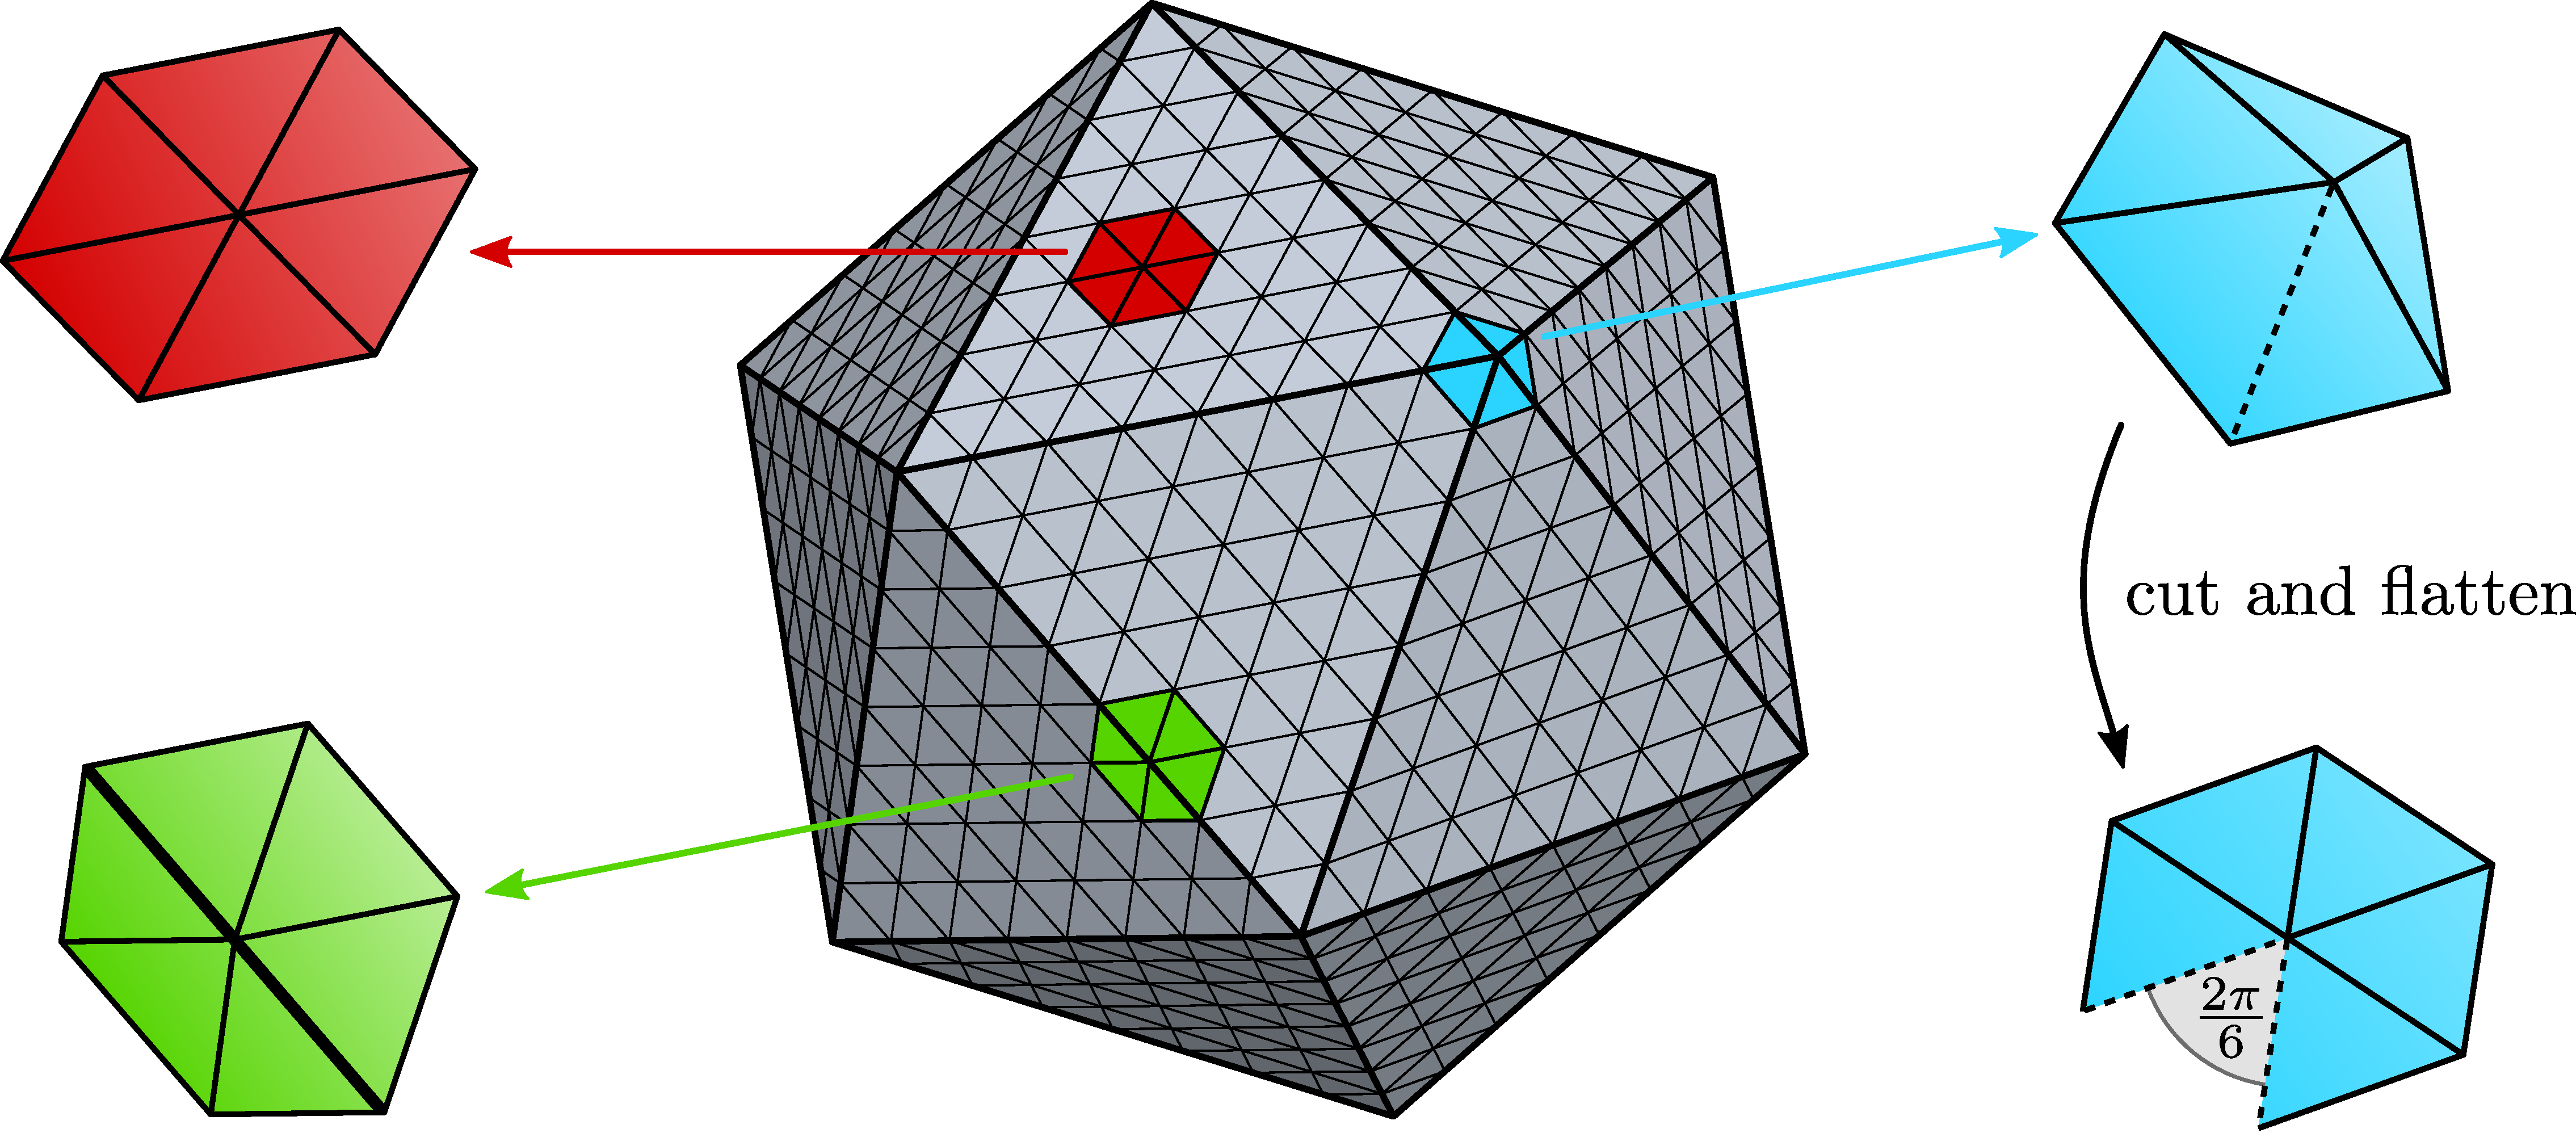
\includegraphics[width=.8\textwidth]{figures/icosahedron_neighborhoods.pdf}
    \vspace*{1ex}
    \caption{\small
        The icosahedron is a Platonic solid that is in \cite{liu2018icoAltAz,gaugeIco2019,zhang2019orientation} used as a piecewise flat approximation of the spherical geometry.
        It consists of 12~vertices, 20~equilateral triangular faces and 30~edges.
        It admits a regular sampling grid, which is constructed by iteratively subdividing each triangle into four smaller triangles.
        After~$r$ iterations, this procedure results in a grid of ${5\mkern-1mu\cdot\mkern-1mu 2^{2r+1} + 2}$ vertices.
        The three highlighted patches show the qualitatively different geometry of neighborhoods around vertices on faces (red), edges (green) and icosahedron vertices (blue).
        The red neighborhood is obviously flat.
        While the green neighborhood is bent in the embedding space, its intrinsic Gaussian curvature is again vanishing.
        That this is the case reflects in the facts that it can be flattened out isometrically (i.e. without being cut) and, equivalently, that the Levi-Civita transport along a closed path around the central node is the identity map.
        The blue neighborhood needs to be cut along one edge in order to be flattened out.
        The angle defect, i.e. the angle by which the cut is spread when flattening the cusp, equals~$\frac{2\pi}{6}$.
        When parallel transporting a vector once around the central vertex of the neighborhood, it gets rotated by this angle defect.
        Instead of having constant positive Gaussian curvature like the sphere $S^2$, the icosahedron's curvature is concentrated (singular) at its vertices and vanishes everywhere else.
    }
    \label{fig:ico_neighborhoods}
\end{figure}


\paragraph{Icosahedral geometry:}
The icosahedron is a discrete two-dimensional manifold consisting of 20~equilateral triangular faces, 12~vertices and 30~edges.
As done for the 2-sphere, we define the icosahedron as being embedded in $\R^3$, from which it inherits the embedding metric in~Eq.~\eqref{eq:spherical_embedding_metric_explicit}.
The embedded tangent spaces $\TpM \subset \R^3$ on the faces are hereby defined such that their normals coincide with the face normals.
Tangent spaces on the vertices and edges could be defined via the average of the adjacent faces' normals as discussed in the following Section~\ref{sec:instantiations_mesh}.
However, as we consider feature fields as being sampled on the icosahedron faces (which is almost everywhere), we are independent form this choice.
Assuming the Levi-Civita connection, % the embedding metric,
the parallel transport of tangent vectors over faces acts such that it keeps them parallel in the embedding space~$\R^3$.
When being parallel transported across an edge, tangent vectors keep the same angle relative to the edge on either side -- this transport may intuitively be thought of as 1) flattening the two adjacent faces out 2) transporting the vector over the edge as usual on a two-dimensional Euclidean space, and 3) bending the two faces back to their original embedding; see Fig.~\ref{fig:transport_mesh} and \cite{craneDiscreteDifferentialGeometry2014}.
Geodesics are therefore piecewise linear in $\R^3$, crossing edges such that their angle of emanation equals their angle of incidence.
Exponential maps $\exp_p(v)$ are thus easily computed by tracing out a piecewise constant path for a distance of $\lVert v\rVert$.
In practice, the authors of~\cite{liu2018icoAltAz,gaugeIco2019,zhang2019orientation} sample feature fields on a regular mesh and consider only those tangent vectors that map to the neighboring mesh vertices.


Fig.~\ref{fig:ico_neighborhoods} shows disc-like neighborhoods around exemplary points on faces (red), edges (green) and vertices (blue) of the icosahedron.
The red neighborhood is fully contained within a face, and is therefore flat.
The green neighborhood is bent in the embedding space, however, its intrinsic (Riemannian or Gaussian) curvature is still zero since the Levi-Civita transport of vectors once around the central vertex preserves them as they are.
That this is the case is equivalent to the fact that the green neighborhood can be flattened out isometrically, i.e. without stretching or cutting it.
This isometric flattening is not possible for the blue type of neighborhoods around vertices, which have to be cut open at one of the edges in order to be flattened out.
Being constructed from five equilateral triangles, the flattened cusp exhibits an angle defect of~$\frac{2\pi}{6}$.
The holonomy of any closed path around any (single) vertex, that is, the angle between an arbitrary vector and its transport once around the loop, is given exactly by this angle defect.
Overall, these results imply that the (discrete) Gaussian curvature of the icosahedron is zero everywhere but at the vertices, where it is singular with holonomy $\frac{2\pi}{6}$.
The simple geometry of the icosahedron allows for it to be cut open and globally flattened out as visualized in Fig.~\ref{fig:ico_cutting}, which was in~\cite{liu2018icoAltAz,gaugeIco2019,zhang2019orientation} used for an efficient implementation of icosahedral $\GM$-convolutions.


The icosahedron's full isometry group $\IsomM = \operatorname{I}_h \leq \O3$ is finite and consists of 120~elements.
It can be thought of as being constructed as the direct product $\operatorname{I} \times \Flip$ of the subgroup $\Flip$ of reflections and the subgroup $\IsomplusM = \operatorname{I} \leq \SO3$ of orientation preserving isometries, containing 60 rotations.
Each vertex~$p$ is stabilized by five discrete rotations around the axis through $p$ and its antipodal vertex, which form the cyclic group~$\C5 \leq \SO2$.
The vertex~$p$ is furthermore stabilized by reflections over the plane defined by the rotation axis and any edge emanating from~$p$, such that its full stabilizer subgroup is given by the dihedral group $\Stab{p} = \D5 \leq \O2$.
The equivariance of icosahedral $\GM$-convolutions w.r.t. isometry groups $\operatorname{I}_h$, $\operatorname{I}$, $\D5$ or $\C5$ was in~\cite{gaugeIco2019} shown to approximate the full $\O3$, $\SO3$, $\O2$ or $\SO2$ equivariance of spherical CNNs reasonably well when continuous rotational data augmentation is used.%
\footnote{
    This was in~\cite{gaugeIco2019} empirically shown for $\operatorname{I} \leq \SO3$.
    That this result generalizes to $\operatorname{I}_h \leq \O3$ is clear since the groups differ only by reflections, w.r.t. which icosahedral $\GM$-convolutions can be made exactly equivariant.
    It holds furthermore for $\D5 \leq \O2$ and $\C5 \leq \SO2$, since these are subgroups of $\operatorname{I}_h \leq \O3$.
}


\begin{figure*}
    \centering
    \begin{subfigure}[b]{0.31\textwidth}
        \centering
        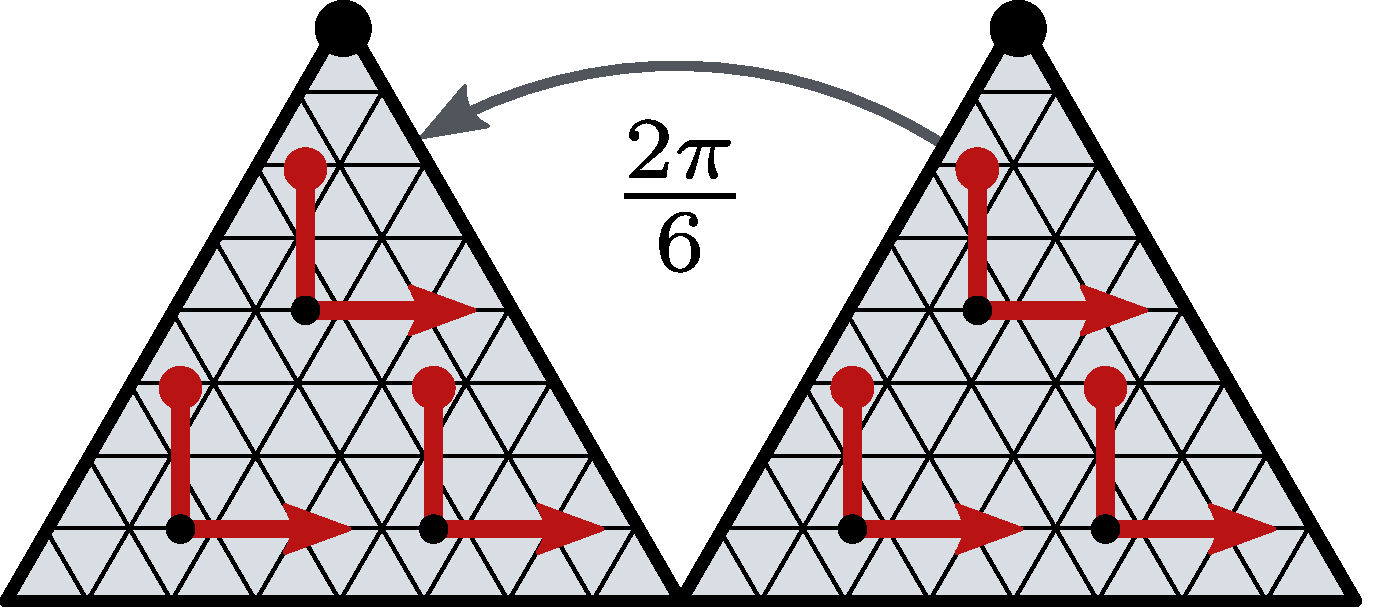
\includegraphics[width=1.\textwidth]{figures/icosahedron_G_structure_1.pdf}
        \vspace*{-6pt}
        \captionsetup{width=.9\textwidth}
        \caption{\small
            Grid-aligned icosahedral $\{e\}$-structure by \citet{liu2018icoAltAz}.
        }
        \label{fig:G_structure_ico_1}
    \end{subfigure}
    \hfill
    \begin{subfigure}[b]{0.31\textwidth}
        \centering
        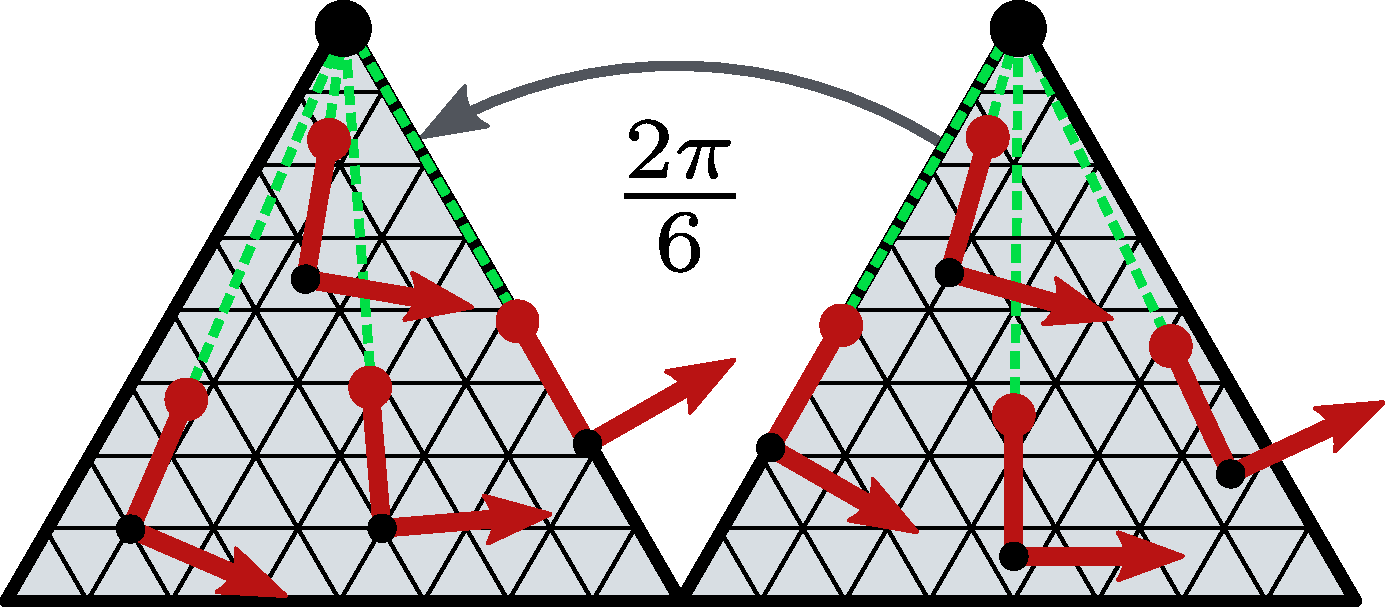
\includegraphics[width=1.\textwidth]{figures/icosahedron_G_structure_2.pdf}
        \vspace*{-6pt}
        \captionsetup{width=.9\textwidth}
        \caption{\small
            North-aligned icosahedral \mbox{$\{e\}$-structure by \citet{zhang2019orientation}}.
        }
        \label{fig:G_structure_ico_2}
    \end{subfigure}
    \hfill
    \begin{subfigure}[b]{0.31\textwidth}
        \centering
        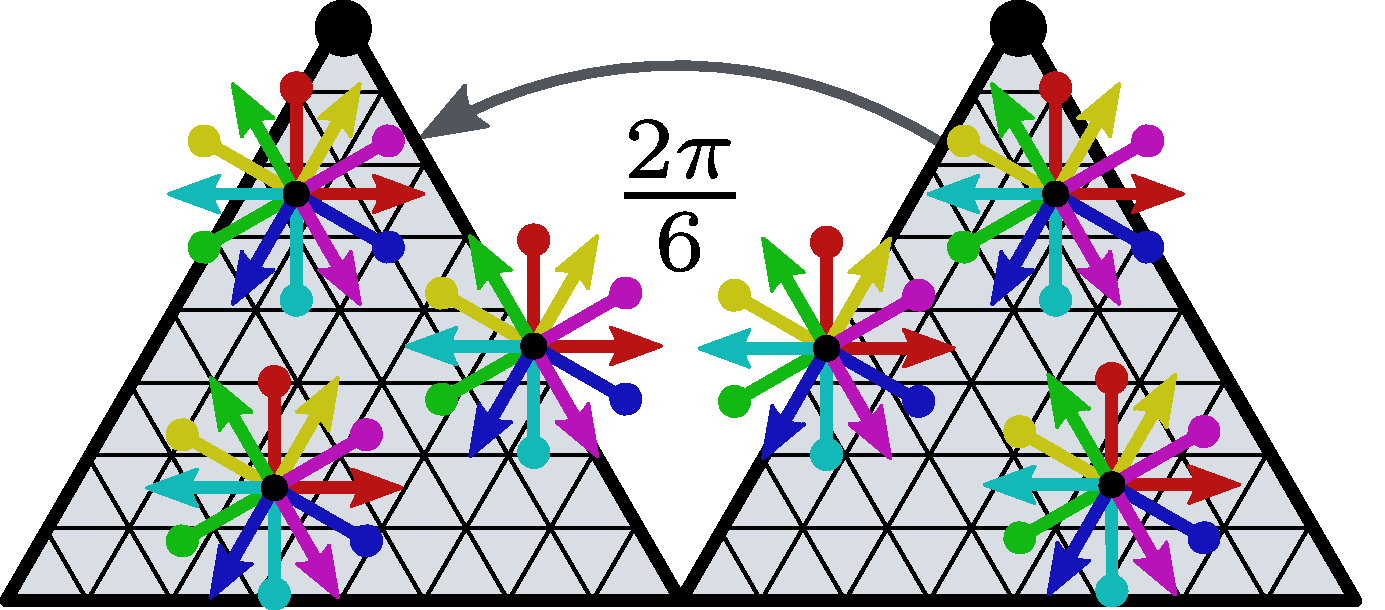
\includegraphics[width=1.\textwidth]{figures/icosahedron_G_structure_3.pdf}
        \vspace*{-6pt}
        \captionsetup{width=.9\textwidth}
        \caption{\small
            Grid-aligned icosahedral $\C6$-structure by \citet{gaugeIco2019}.
        }
        \label{fig:G_structure_ico_3}
    \end{subfigure}
    \caption{\small
        Conceptual idea of the $G$-structures assumed in~\cite{liu2018icoAltAz,zhang2019orientation,gaugeIco2019}.
        For space reasons, only two adjacent faces next to the north pole of the flattened icosahedron (Fig.~\ref{fig:ico_cutting}) are shown.
        The $\{e\}$-structure in Fig.~\ref{fig:G_structure_ico_1} is defined by aligning all frames along the ``horizontal'' edges of the faces (assuming the polar axis to be vertical).
        Fig.~\ref{fig:G_structure_ico_2} shows an alternative $\{e\}$-structure whose frames are aligned towards the north pole.
        It is in contrast to the previous $\{e\}$-structure continuous since frames on the cut edges agree with each other when gluing the edges back together.
        The $\C6$-structure in Fig.~\ref{fig:G_structure_ico_3} is constructed by adding frames that are rotated by multiples of $\frac{2\pi}{6}$ to the $\{e\}$-structure from Fig.~\ref{fig:G_structure_ico_1}.
        Since this angle agrees with the angle defect at the cut edges, the thus defined $\C6$-structure is smooth (continuous).
        Note that the two $\{e\}$-structures are incompatible with (i.e. not closed under) the Levi-Civita transport but imply an alternative trivial connection.
        The $\C6$-structure, in contrast, is compatible with the Levi-Civita transport.
     }
    \label{fig:G_structures_ico}
\end{figure*}


\paragraph{Icosahedral \textit{G}-structures:}
The icosahedral $\GM$-convolutions by~\citet{liu2018icoAltAz} and~\citet{zhang2019orientation} (implicitly) assume $\{e\}$-structures, while that by~\citet{gaugeIco2019} assumes a $\C6$-structure.
Fig.~\ref{fig:G_structures_ico} visualizes the idea behind these $G$-structures, which we explain in the following three paragraphs in more detail.


The $\{e\}$-structure by~\citet{liu2018icoAltAz}, shown in Fig.~\ref{fig:G_structure_ico_1}, is defined by aligning the first frame axes with the ``horizontal'' edges of the corresponding triangular faces.
When flattening the icosahedron into a plane as shown in Fig.~\ref{fig:ico_cutting}, all frames of this $\{e\}$-structure are parallel in this plane, which greatly simplifies the implementation of the corresponding $\GM$-convolutions.
As usual, the $\{e\}$-structure specifies a unique trivial connection according to which features are transported.
This trivial connection agrees within the faces, on edges which are not cut in Fig.~\ref{fig:ico_cutting} and on the magenta cut edge with the Levi-Civita connection.
However, its transport over the remaining cut edges differs from the Levi-Civita transport since the frames of the $\{e\}$-structure rotate there discontinuously by an angle of~$\frac{2\pi}{6}$.
As the $\{e\}$-structure is preserved by rotations in $\C5$ around the polar axis, its $\GM$-convolutions are approximately $\SO2$-equivariant, i.e. approximate the models from the previous Section~\ref{sec:spherical_CNNs_azimuthal_equivariant}.
However, the $\{e\}$-structure -- and therefore the network inference -- is \emph{non-continuous} over the edges with non-zero angle defect.
Furthermore, the reference frames do not point exactly towards the north pole, as it is the case for the spherical $\{e\}$-structure from Section~\ref{sec:spherical_CNNs_azimuthal_equivariant} and Fig.~\ref{fig:G_structure_S2_2}.


\citet{zhang2019orientation} propose to resolve the latter two issues by working with the $\{e\}$-structure in Fig.~\ref{fig:G_structure_ico_2}.
It is defined such that the frames point exactly along the projection of the polar axis onto the faces, i.e. towards the north pole.
This $\{e\}$-structure is continuous everywhere except at the north and south poles.%
\footnote{
    To see this, imagine to glue the cut edge in Fig.~\ref{fig:G_structure_ico_2} back together:
    the frames on the left and right half of the edge are then being mapped together, which is not the case in Fig.~\ref{fig:G_structure_ico_1}.
}
It is in this sense a better approximation of the spherical $\{e\}$-structure from Fig.~\ref{fig:G_structure_S2_2}.
The $\{e\}$-structure implies again a unique trivial connection.
Its transport agrees with the Levi-Civita transport over edges, however, it differs from it when transporting over faces since it rotates vectors smoothly along with the frames.
As the other $\{e\}$-structure, this frame field is invariant under azimuthal rotations in $\C5$, and approximates thus azimuthal rotation equivariant spherical CNNs.


The $\C6$-structure in Fig.~\ref{fig:G_structure_ico_3} by~\citet{gaugeIco2019} is defined by augmenting the frames of the $\{e\}$-structure from Fig.~\ref{fig:G_structure_ico_1} with those frames that are rotated by multiples of $\frac{2\pi}{6}$.
It is clearly continuous since the angles between the set of preferred frames at each point equal exactly the angle defects at the cut edges.
It is in contrast to the previous two $\{e\}$-structures compatible with the Levi-Civita transport since the structure group $\C6$ agrees with the icosahedron's holonomy group.
The $\C6$-structure is furthermore preserved under the action of the icosahedron's orientation preserving isometries $\operatorname{I}$.
$\GM$-convolutions on this $\C6$-structure approximate therefore the fully $\SO3$ rotation equivariant spherical CNNs from Section~\ref{sec:spherical_CNNs_fully_equivariant}.

\begin{figure}
    \centering
    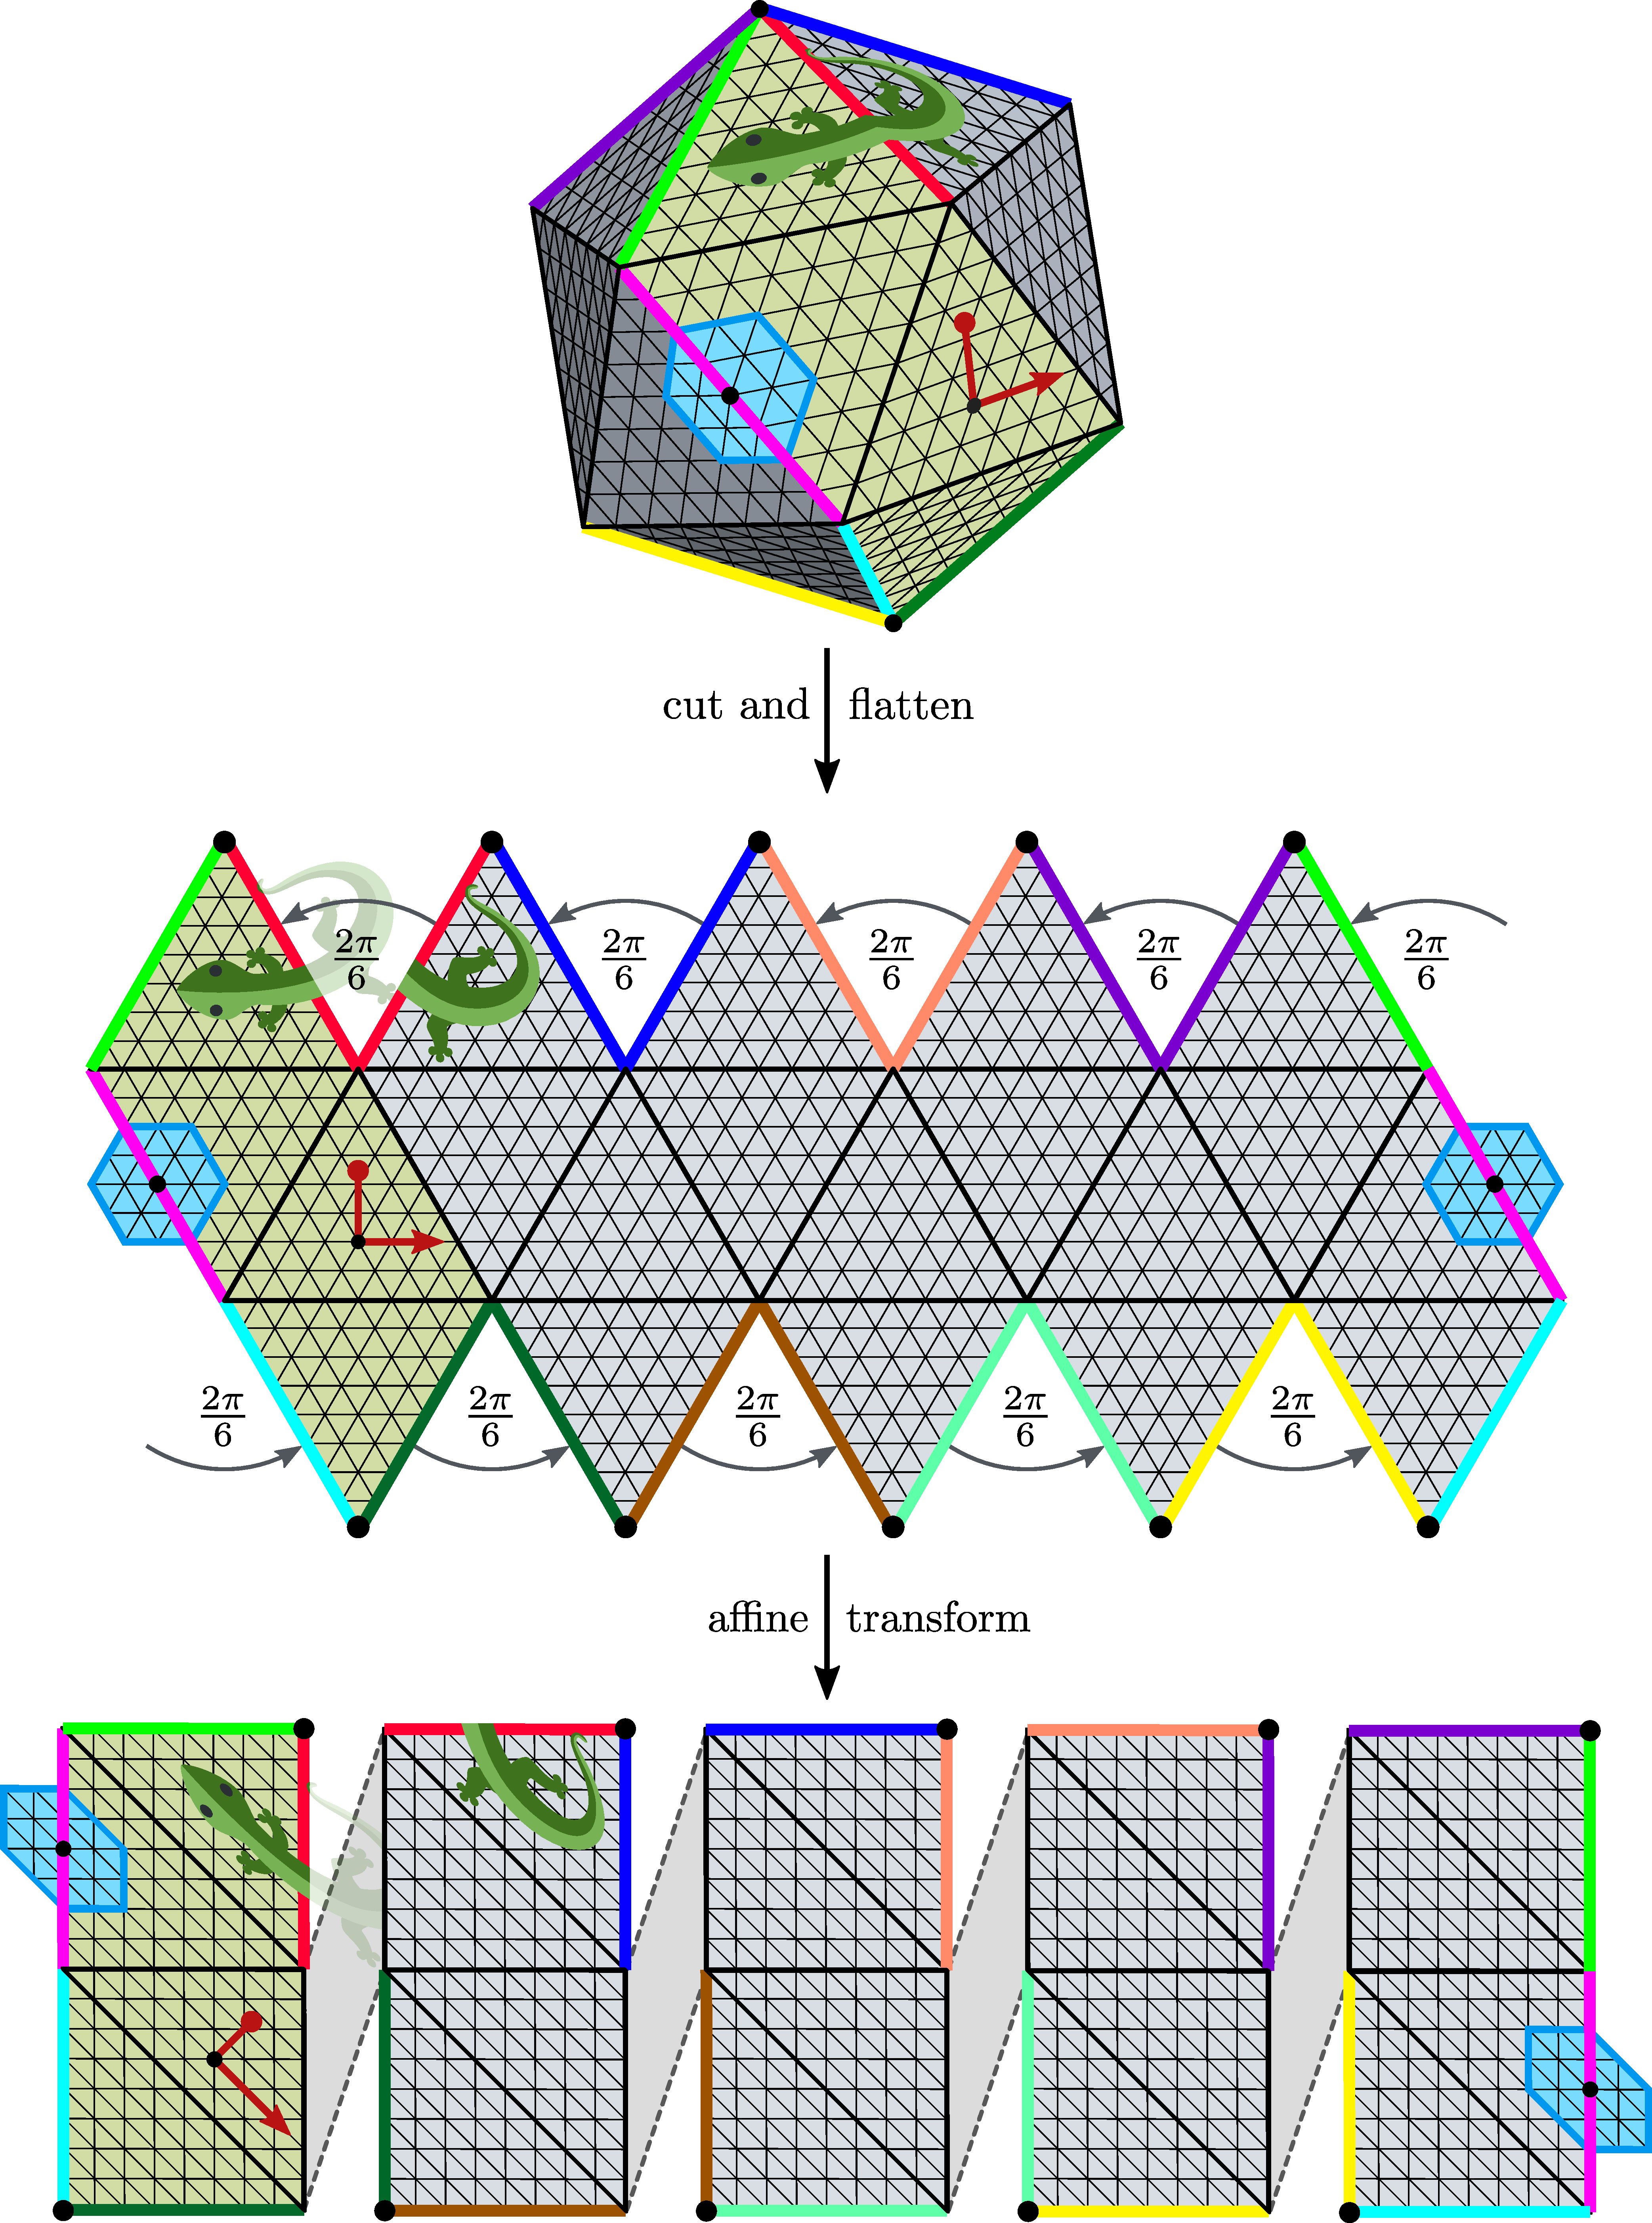
\includegraphics[width=.9\textwidth]{figures/icosahedron_cutting.pdf}
    \vspace*{1.5ex}
    \caption{\small
        The implementations in \cite{liu2018icoAltAz,gaugeIco2019,zhang2019orientation} represent feature fields relative to an atlas that covers the icosahedron with five charts.
        To construct these charts, one cuts the icosahedron along the colored edges and flattens it out.
        Five regions, consisting of four triangles each, are then sheared to rectangular chart codomains.
        This operation maps the hexagonal grid to a grid of square pixels, such that icosahedral feature fields can be encoded by a set of five rectangular arrays.
        Note that reference frames and kernels are deformed accordingly on the chart codomains.
        The Levi-Civita transport over all colored edges but the magenta one picks up a rotation of $\pm\frac{2\pi}{6}$, with the sign depending on the transport direction.
        This is implemented by transport padding rows of pixels along the cut edges as previously described in Fig.~\ref{fig:mobius_conv_numerical}.
        {
        \\ \color{gray} \scriptsize
            (Lizards adapted under the Creative Commons Attribution 4.0 International
            \href{https://github.com/twitter/twemoji/blob/gh-pages/LICENSE-GRAPHICS}{\underline{license}}
            by courtesy of Twitter.)
        }
     }
    \label{fig:ico_cutting}
\end{figure}


\paragraph{Implementations:}
To implement the $\GM$-convolutions on the corresponding $G$-structures,
\citet{liu2018icoAltAz}, \citet{zhang2019orientation} and~\citet{gaugeIco2019}
assume a regular grid on the icosahedron's faces; see Fig.~\ref{fig:ico_neighborhoods}.
This regular hexagonal grid is constructed by iteratively subdividing edges, replacing each triangle with four smaller ones.
At resolution~$r$, this yields a grid with ${5\mkern-1mu\cdot\mkern-1mu 2^{2r+1} + 2}$ vertices.
Note that this grid is by construction exactly symmetric under isometries of the icosahedron, which leads to an exact $\IsomGM$-equivariance of the discretized $\GM$-convolutions.%
\footnote{
    The icosphere grid, used by some of the models from Sections~\ref{sec:spherical_CNNs_fully_equivariant} and~\ref{sec:spherical_CNNs_azimuthal_equivariant}, is defined by projecting the nodes of this grid to unit radial distance from the origin, i.e. to~$S^2$.
    The models in this section do not assume this projection but convolve directly over the piecewise flat icosahedral geometry.
}
\citet{liu2018icoAltAz} proposed to represent icosahedral feature fields relative to the atlas of charts that is shown in Fig.~\ref{fig:ico_cutting}.
The charts have the advantage that they map the hexagonal grids on the icosahedron's faces to common square pixel grids.
Note, however, that orthonormal frames on the icosahedron are in this representation deformed, such that they are not orthonormal relative to the canonical Euclidean metric.
Hexagonal convolution kernels on the icosahedron are deformed accordingly and can be implemented in terms of square kernels which are masked such that two of their corners are filled with zeros.


The $\GM$-convolution by~\citet{liu2018icoAltAz} assumes frames that are all parallel and can therefore in the interior of the charts, where the kernel support does not extend over its boundaries, be implemented via a conventional Euclidean convolution.
At points that are close to an edge between different charts, the kernel accumulates features from beyond the cut.
As already discussed and visualized in Section~\ref{sec:mobius_experiment_main} and Fig.~\ref{fig:mobius_conv_numerical}, this is conveniently implemented via a transport padding operation which pads a border of parallel transported features around the array of square pixels before running the convolution operation.
For the trivial transport implicitly assumed by~\citet{liu2018icoAltAz}, this padding operation just copies a row of features at each edge without transforming them.
Since the authors assume the trivial structure group $G=\{e\}$, the hexagonal kernels remain unconstrained.


The implementation of~\citet{gaugeIco2019} is mostly similar, however, it differs crucially in that it uses Levi-Civita transporters and $\C6$-steerable kernels.
Instead of directly padding rows of pixels across edges, the Levi-Civita transport requires that the features are steered either by $g=e$ for all internal edges and the magenta edge or by an angle of $\pm\frac{2\pi}{6}$ over all edges with angle defect $\frac{2\pi}{6}$, with the sign depending on the transport direction.
\citet{gaugeIco2019} assume the regular representation of~$\C6$ as field type and constrain the convolution kernels to satisfy the corresponding steerability constraint.
After transport padding, their $\GM$-convolution is implemented as a conventional Euclidean convolution with these steerable kernels.
Note that this $\GM$-convolution is within the faces, i.e. except for the transport padding, similar to the HexaConv by \citet{Hoogeboom2018-HEX}.


Since the $\GM$-convolution by~\citet{zhang2019orientation} assumes a trivial structure group $G=\{e\}$, the transport padding is again implemented as a trivial copy of pixels without steering and the kernels are again left unconstrained.
However, as the frames of the $\{e\}$-structure are aligned towards the north pole, they are not longer parallel in the rectangular square pixel representation, which prevents an immediate implementation in terms of conventional convolutions.
Instead, the kernels have to be applied in a different rotation at each grid point.
As the hexagonal kernel can be rotated by $\frac{2\pi}{6}$ without using interpolation, and since the alignments towards the north pole differ at most by this angle from each other, the authors propose the following efficient approximating of this operation:
they convolve twice on each face, once with the original kernel and once with its $\frac{2\pi}{6}$ rotated version.
The two response fields are then linearly combined, with the precomputed interpolation weights depending on the angles of the north-aligned reference frames relative to the two kernel alignments (i.e. relative to the pixel grid).
This implementation is therefore approximately twice as costly as those in~\cite{liu2018icoAltAz,gaugeIco2019}.


An alternative implementation of spherical convolutions on the icosahedron was proposed by~\citet{eder2020tangent}.
The authors project the spherical signal on planes spanned by the 20 faces (denoted as tangent images) and subsequently run a conventional CNN on each of these images.
We did not include this network in our list as it processes these representations independently from each other, that is, it does not transport or pad features between them, and is therefore not exactly described as $\GM$-convolution.


As mentioned before, the empirical results by~\citet{kicanaoglu2019gaugeSphere} suggest that the icosahedral geometry approximates the spherical geometry reasonably well for deep learning applications.
More specifically, the authors compare their spherical CNN on an icosphere grid with the piecewise flat icosahedral CNN by~\citet{gaugeIco2019} and find that both perform similarly despite the deformed geometry of the latter.
The equivariance of icosahedral CNNs under continuous rotations in $\SO3$ is found to be violated significantly, however, this seems to be a mere overfitting effect as it is easily and without loss of model performance counteracted by leveraging $\SO3$ data augmentation.


As always, we want to mention that the $\C5$-equivariant CNNs by \citet{liu2018icoAltAz} and \citet{zhang2019orientation} can easily be made $\D5$-equivariant by considering a $\Flip$-structure and thus reflection-steerable kernels.
Similarly, the $\operatorname{I}$-equivariant CNN by \citet{gaugeIco2019} can be made equivariant under the full isometry group $\operatorname{I}_h$ of the icosahedron by making the kernels $\D6$-steerable instead of $\C6$-steerable.
